\section{Subroutines and the Stack}

\section*{Subroutine Call and Return}
\begin{itemize}
  \item Label with Name (MulBy3)
  \item Return Statement (BX $1 R$ )
\end{itemize}

\begin{center}
\begin{tabular}{lllll}
00000050 & 4604 & MulBy3 & MOV & R4,R0 \\
00000052 & 0040 & LSLS & RO, \#1 &  \\
00000054 & 4420 & ADD & R0,R4 &  \\
00000056 & 4770 & BX & LR &  \\
\hline
\end{tabular}
\end{center}

Stack

\begin{itemize}
  \item Stack Area (Section)
  \item Stack Pointer (SP)
  \item PUSH \{...\}
  \item POP \{...\}
  \item Direction on ARM
  \item Alignment
  \item Only words
\end{itemize}

Continuous area of RAM\\
R13 $\rightarrow$ points to last written data value\\
Decrement SP and store words\\
Read words and increment SP\\
full-descending stack\\
word-aligned\\
32-Bit

\section*{Stack - Push and Pop}
\begin{itemize}
  \item Number of Pushs = Number of Pops
  \item Stack-limit < SP < stack-base\\
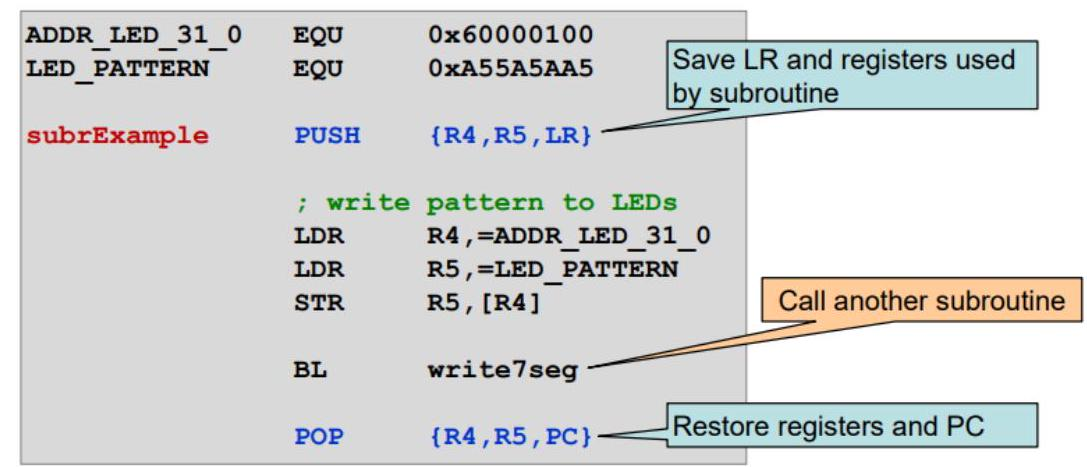
\includegraphics[max width=\textwidth, center]{2024_12_29_79e6b22f503fb7b4f718g-08}
\end{itemize}

PUSH \{R2,R3,R6\}

\begin{center}
\begin{tabular}{llll}
00000000 & B083 & SUB & SP,SP,\#12 \\
00000002 9200 & STR & R2,[SP] &  \\
00000004 & 9301 & STR & R3,[SP,\#4] \\
000000069602 & STR & R6,[SP,\#8] &  \\
\end{tabular}
\end{center}

\section*{POP \{R2,R3,R6\}}
\begin{center}
\begin{tabular}{|llll|}
\hline
00000008 9A00 & LDR & R2,[SP] \\
0000000A 9B01 & LDR & R3,[SP,\#4] \\
0000000C 9B02 & LDR & R6,[SP,\#8] \\
0000000E B003 & ADD & SP,SP,\#12 \\
\hline
\end{tabular}
\end{center}